\section{Instrument}
\label{sec:Instrument}

\subsection{Design Considerations and Sensitivity} 
\label{sec:DesignConsiderations}  

To achieve the scientific and technical goals of \name, we must be able to demonstrate atmosphere-limited performance of the telescope and detectors, and be able to make both pointed observations toward specific objects and small-area maps to validate the sensitivity.  The goal is to detect galaxies with $0.5 < z < 1.5$ in \cii, which sets the wavelength range to 240 - 420 \mum.

The design should be such that the sensitivity of the instrument is
limited by the photon noise of the atmosphere and optics.
%Balloons make attractive platforms for far-IR measurements because of 
%the greatly reduced emissivity and absorption from the atmosphere To 
%take advantage of this, we must design the instrument and optics to 
%have lower noise than the expected atmosphere emission The 
%requirements for a dispersive spectrometer are much more stringent in 
%this regard than for a continuum instrument due to the much smaller 
%bandwidth per detector. 
%The atmosphere will limit the sensitivity in two ways: first, by the 
%background loading, and second by fluctuations in line emission which 
%may mimic a spectroscopic signal Here we only treat the effects of 
%the former; the latter is dealt with by our scanning modulation 
%(Section \ref{sec:Observing}) to remove spatial and temporal 
%fluctuations  
To estimate the atmosphere background, the (proprietary) ATM model of 
Juan Pardo was used.  We have assumed 
%The results for the $T_{RJ}$ of the atmosphere from 50 to 750 \mum\ are shown assuming  
a flight at mid-latitudes, an altitude of 37 km, and 
observations at 45\arcdeg\ elevation.  The ATM model calculates the 
opacity due to all relevant atmospheric species. 
%The antenna temperature is less than 1 K over 75\% (89\%) of the band 
%at 30 (37) km altitude.  
We calculate the noise equivalent power (NEP) due to photon shot noise 
from a greybody with physical temperature $T$ and emissivity 
$\epsilon_\nu$ being detected by a system with optical efficiency 
$\eta$ as 
\begin{eqnarray} 
\label{eq:nep_shot} 
{\rm NEP}_\gamma = \sqrt{\frac{N_{pol}}{2}}2 h \nu \sqrt{n(n+1) \Delta \nu} & , &  
n = \frac{\eta \epsilon_\nu}{\exp{(h \nu / k T)} - 1} 
\end{eqnarray} 
where $n$ is the photon occupation number  
%The two dominant sources 
%of photon shot noise for \name\ are the telescope optics and the 
%atmosphere In order that the photon shot noise limit the instrument 
%performance,  
The detector NEP must be less than the noise NEP$_\gamma$.  
%For
%bolometers, whose noise is dominated by the phonon noise in their
%thermal conductance $G$ to the bath, this is $ {\rm NEP}_{G} = \sqrt{k
%T^2 G} < {\rm NEP}_\gamma$. 
The low noise detectors we will use for
\name\ are discussed in Section \ref{sec:Detectors}. The final figure
of merit for detecting an unresolved line in a point source is given
by the line sensitivity
\begin{equation} 
{\cal S}_\gamma = \frac{2}{N_{pol}}\frac{\sqrt{2} {\rm NEP}_\gamma} 
{\eta_{opt} A_{eff} \rm{e}^{-\tau_\nu}} \; \;
\left[{\rm \frac{W}{m^{2}}~\sqrt{sec}}\right]
\end{equation} 
where $\tau_\nu$ is the atmosphere optical depth, related to the
emissivity as $\epsilon_\nu = 1 - \exp{(-\tau_\nu)}$.  The effective
collecting area, $A_{eff}$, of the telescope is decreased from the
geometrical value $A = \pi (D_{tel}/2)^2$ by
%two factors, the surface 
%efficiency 
%\begin{equation} 
%\eta_{surf} = \exp{(-(4 \pi \sigma_{surf}/ \lambda)^2)} 
%\end{equation} 
%and  
the illumination of the optics.

We have have considered the performance of various potential
architectures for \name, incorporating the atmospheric transmission
and loading, a range of telescope sizes, and the possibility of
actively cooling the telescope to minimize its thermal emission.
While a cooled aperture performs better, it is very costly for a given
aperture size, and the performance improvement is modest because even
a balloon altitudes there is $\sim$1\% emission from the 250~K
atmosphere.  In light of these calculations, and our experience with
ballooning with \blast\ \Citep{devlin04,pascale08} and spectroscopy
with Z-Spec \Citep{inami08,earle06,bradford04,bradford03,naylor03}, we
have arrived at a \D\ off-axis ambient-temperature telescope, with
carefully controlled illumination to avoid spillover to warm surfaces.
These parameters and sensitivity factors for our design are given in
Table \ref{tab:Parameters}.

For optimal sensitivity to line emission in distant galaxies, the
spectral resolving power $R \equiv \lambda/\Delta \lambda$ should be
matched to the line width. 
%For \name, we are attempting to achieve a
%balance between sensitivity to invidual objects and to the power
%spectrum; 
For the relatively massive galaxies we are targeting, a resolution $R = 450$ (670 \kms) is adequate: higher resolution increases the number of detectors required and may over-resolve the line.
%in order to ease the requirement on the detector NEP
%(insuring that the system is strongly background limited), and to
%reduce the detector count. 
In principle, the required spectral resolution and large area mapping
could be achieved with either a Fabry-Perot (FP) or FTS spectrometer
design. However, both of these require a moving component, and both
incur sensitivity penalties.
%for follow-up of sources with known
%positions. 
The FP does not cover the entire frequency range instantaneously and
must be scanned, and the FTS places the full optical bandwidth of the
entire band on each detector, increasing the noise. The best approach
is a reflective, blazed diffraction grating, which offers large
instantaneous bandwidth and good sensitivity.
%, with no moving
%parts. 

\subsection{Spectrometer Architecture} 
\label{sec:Spectrometer} 

To achieve integral-field spectroscopy over a 2-D field, the spectrometer optics begin by slicing a $5\times5$ pixel field to form 
a 25 pixel long pseudo-slit, which feeds the spectrometer. 
For optimal efficiency, two independent spectrometer
modules and image slicers with separate fields of view are combined to
cover the full 240-420 \mum\ range: a short wavelength module covering
240-317 \mum, and a long wavelength module covering 317-420 \mum. The slicing
optics follow the same design as successfully implemented in the PACS and
FIFI-LS spectrometers \citep{looney03apj,looney03spie}; see Figure \ref{fig:Slicer}. 

In Figure \ref{fig:SpectrometerModule} we show the long wavelength spectrometer module. A powered mirror collimates the light passing through the pseudo-slit, and forms an image of the telescope aperture on the grating. The grating itself serves
as a cold pupil that controls the telescope illumination. The grating is
operated in first order, and is sized to provide a slit-limited resolving
power of $R=450$. A second powered mirror then focuses the dispersed light
onto the focal plane. The long wavelength module has a size of $60 \times 32 \times
22$~cm; the linear dimensions of the short wave module are a factor of
1.3 smaller.

The simple spectrometer design employed here produces a moderate amount of
anamorphic magnification, such that the image of a spectrally unresolved
source is stretched in the dispersion direction by 20-50\%. We will use a
hexagonal array of pixels in which the pitch in the dispersion direction
is naturally 15\% larger than in the spatial direction, partially
countering this anamorphism. The final imaging in the long wave module is
at f/2.4, such that an image of a point source is 0.91mm in size. We
design our hexagonal array of microlenses to have a pitch in the spatial
direction of 1.18mm, such that we slightly undersample the spatial
resolution element, and oversample the spectral resolution element. With a
25x64 pixel array we achieve an instantaneous bandwidth of $\approx$$14\%$
for each of the 25 spatial positions, and 2 grating settings (with the
grating tipped by 5.5 degrees) are sufficient to cover the entire
$\approx$$28\%$ band. The short wave module is imaged at f/3.3 to maintain
a constant image size, and the same array of hexagonally packed
microlenses will be used to cover this band.
 
Both spectrometer modules are contained within a 1 K optical approximately cavity approximately 70 cm in diameter and 25 cm tall, painted black on the inside and using black baffles to control stray light and keep loading on the detectors low. Light enters this cavity after passing through low pass filters at 77K, 40K, and 4K, with a capacitive mesh bandpass filter at its entrance.  IR blocking
filters between each of the low pass filters cut down on the loading
and increase the cryogen hold time.  The total size of the spectrometer optics leads to a a cryostat of only slightly large overall size and cryogenic volume as the Z-Spec cryostat.
 
\begin{figure}[t]
  \begin{tabular}{lc}
    \begin{minipage}{3.5in}	
	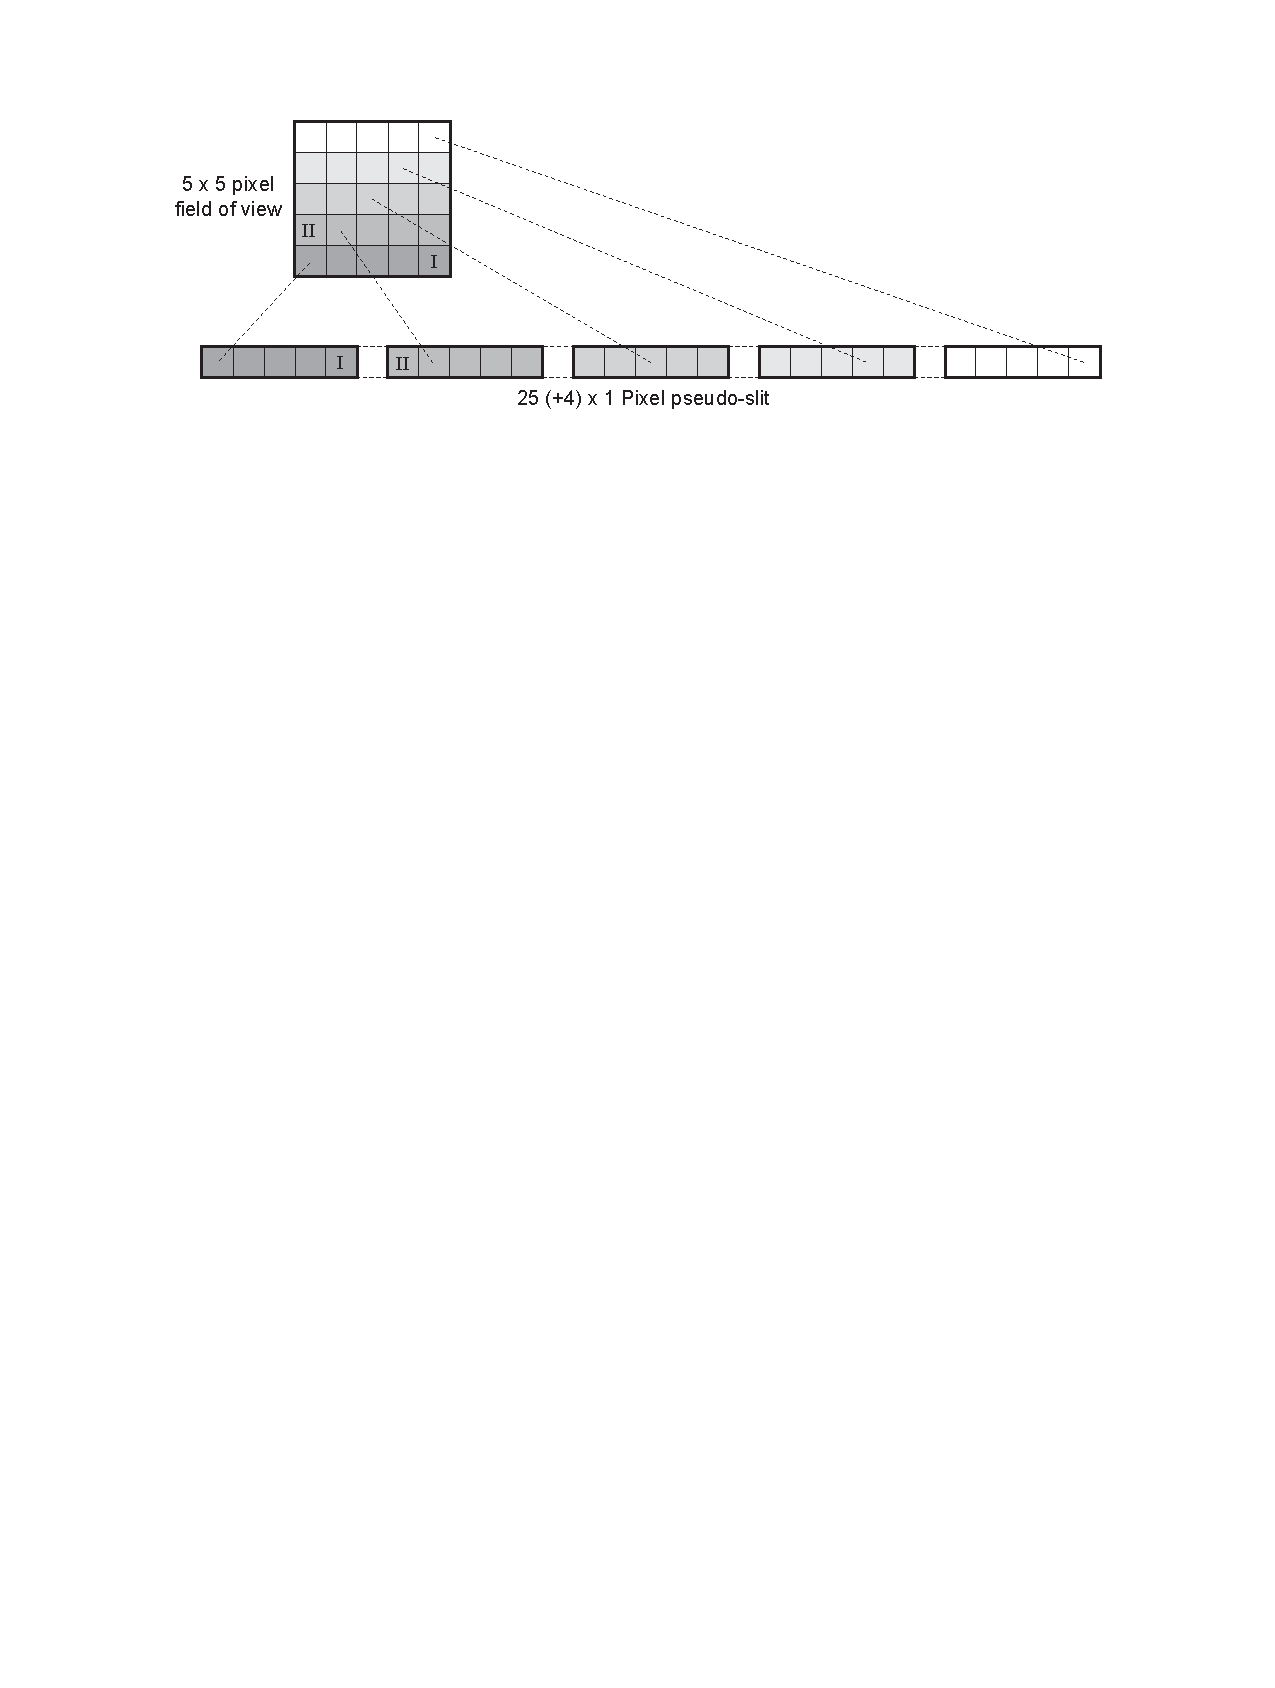
\includegraphics[width=3.5in]{slit_mapping.pdf}
	\captionbaseline\caption{\small {\it Right:} The image slicing optics, which present a long pseudo-slit to the spectrometer. {\it Above :} The mapping of the 2-D focal plane to a single long pseudo-slit.  These figures adapated from \citet{looney03apj} for the design of FIFI-LS.}\label{fig:Slicer}
    \end{minipage} &	
 \begin{minipage}{3in	}
      \begin{center}	
	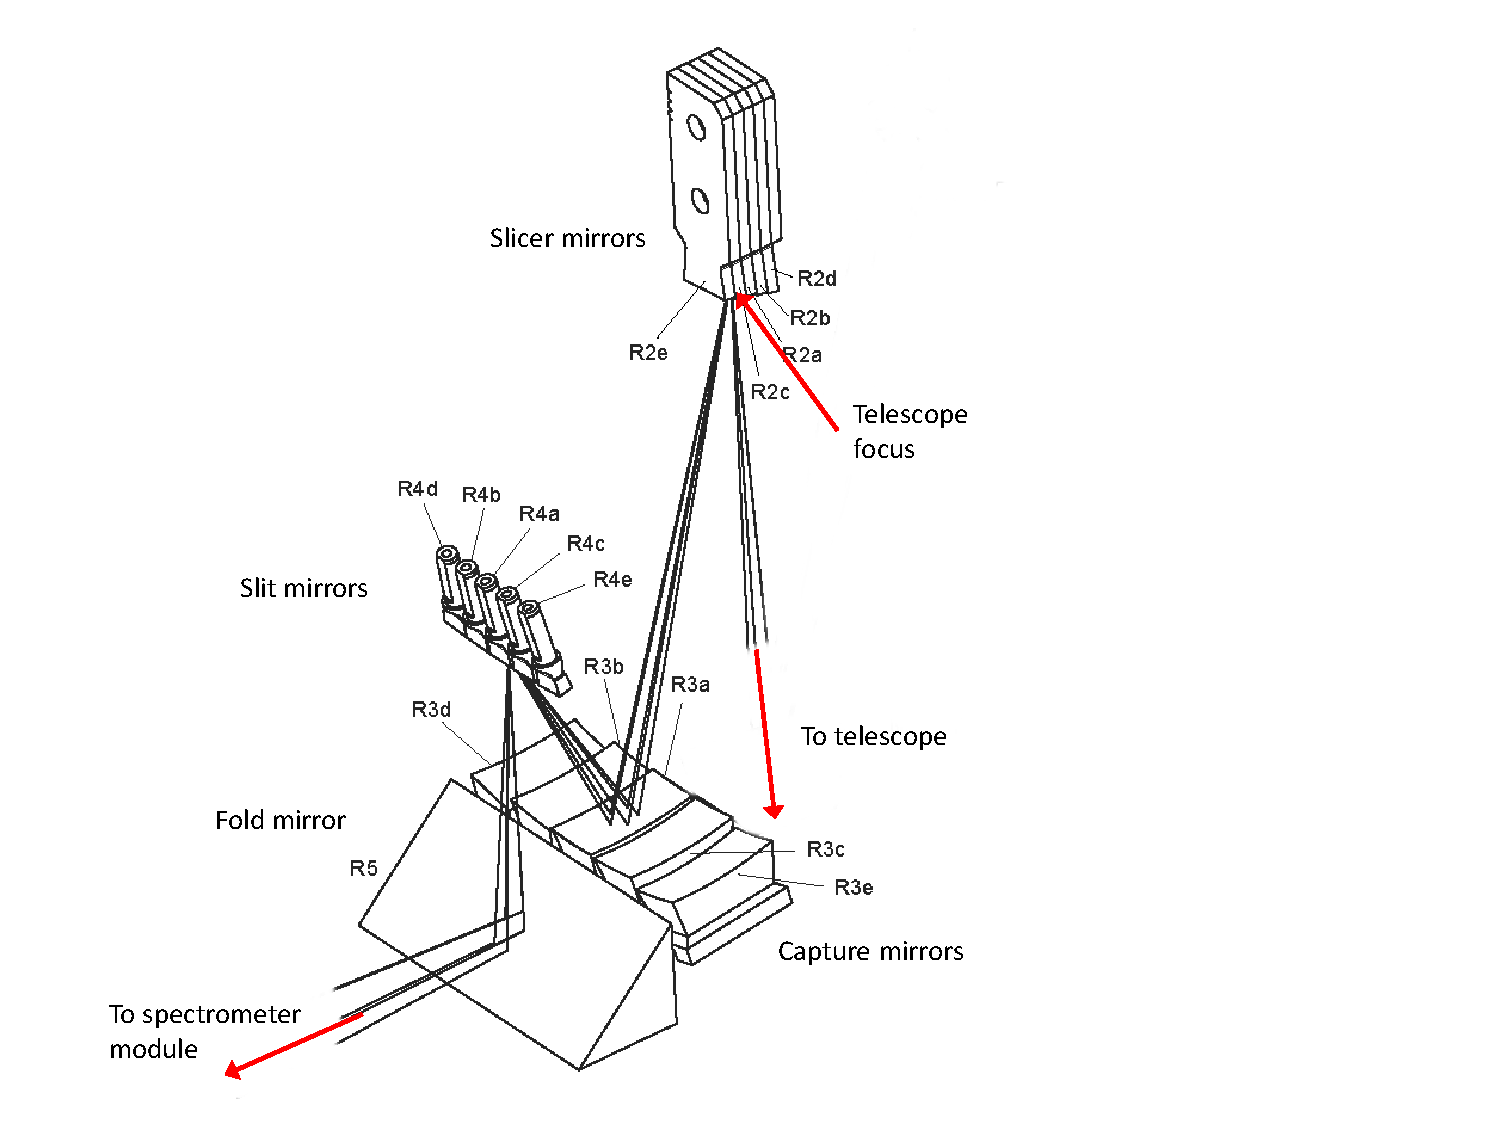
\includegraphics[width=3in]{image_slicer_adapted.pdf}
     \end{center}	
   \end{minipage} 
%   \begin{minipage}{2in}
 %  \end{minipage}
  \end{tabular}
\linefig
\end{figure}

\begin{figure}[t]
\vspace{0.35in}
  \begin{center}
    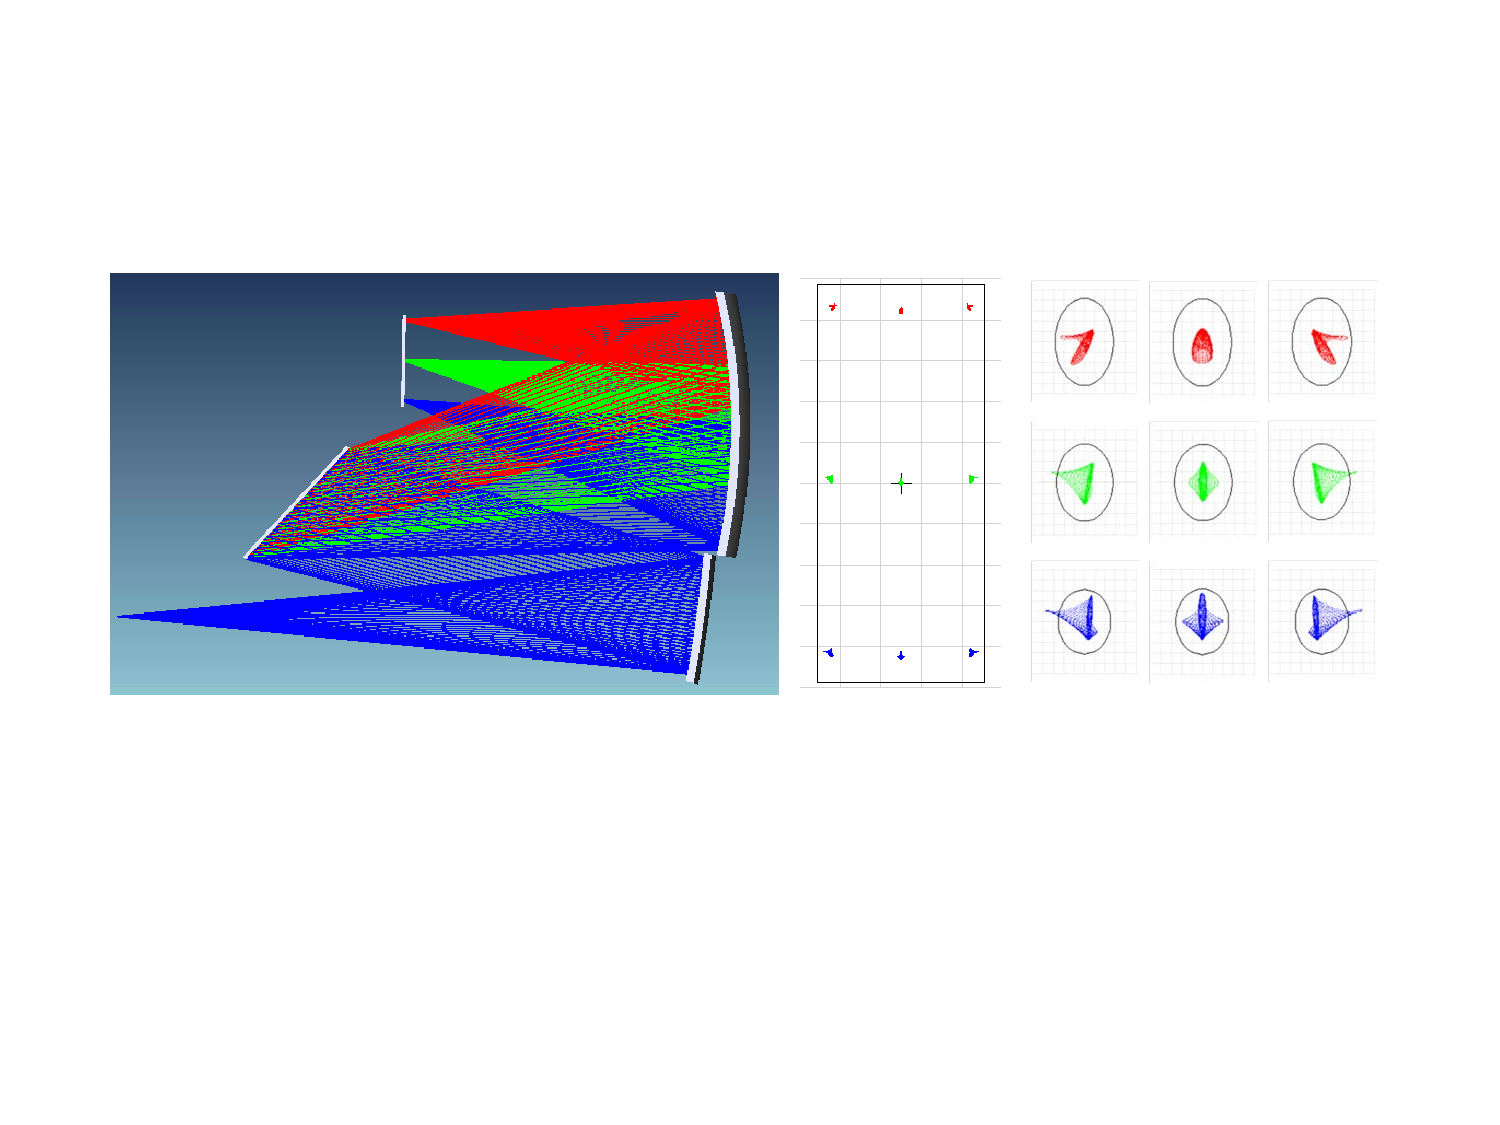
\includegraphics[width=6.5in]{starfire_spectrometer.pdf}
    \captionbaseline\caption{\small {\it Left:} The long wave spectrometer module showing the dispersion and imaging for 3 wavelengths spanning the instantaneous bandwidth. {\it Center:} Image of the array for the 3 wavelengths, and 3 field positions spanning the 25 pixel slit. \R\ Geometric spot sizes for the 9 beams, compared with diffraction-limited Airy disk.}
    \linefig\label{fig:SpectrometerModule}
  \end{center}
\end{figure}

\subsection{Kinetic-Inductance Detector (KID) Arrays}  
\label{sec: Detectors} 

KIDs have emerged in the last decade as a straightforward approach to very large detector arrays for astrophysics.  These devices rely on thin-film, high-Q micro-resonators that absorb incident radiation and respond by changing resonance frequency and line-width.  These changes may be monitored by measuring the complex (amplitude and phase) transmission of an RF or microwave tone tuned to the resonance frequency.  % The response is linear as long as changes in the loading are small.  
Due to the high resonance quality factors (narrow line widths) that can be achieved, large numbers of KIDs may be read out on a single RF/microwave feed line, and the only cryogenic electronics necessary is a single cold (4--20~K) RF/microwave amplifier per transmission line, which may be used for amplifying the signals of thousands of detectors.

KID technology is now approaching the performance levels of the SQUID-multiplexed bolometer systems in ground-based instruments.  One example is the MUSIC camera now at the Caltech Submillimeter Observatory (CSO) \cite{Schlaerth_10} with participation from collaborator J.\ Zmuidzinas, with a total of 2304 detectors in 4 wavelength bands.  Another is the dual-band 150/240~GHz, 224-pixel NIKA camera fielded at the IRAM 30-m telescope by European groups at SRON Utrecht (Baselmans), Institut NEEL (Benoit), and Cardiff (Doyle), which has demonstrated sensitivities approaching the photon background limit  \citep{Monfardini_11, Yates_11,Calvo_13}. 
KID technology has benefitted greatly from the Caltech / JPL discovery of the outstanding properties of titanium nitride (TiN) \cite{LeDuc_10}.   TiN has a high normal state impedance, making it easy to lithograph inductors into direct absorbers.  It has intrinsically high Q values---sQs as high as $3\times10^{7}$ have been achieved with TiN resonators.  These high Qs translate into the ability to build sensitive devices, and NEPs as low as $4\times10^{-19}\,\rm W\,Hz^{-1/2}$ have been measured at Caltech / JPL,  well below the \icaris\ requirement of NEP$_{\rm BG}\sim2\times10^{-18}\,\rm W\,Hz^{-1/2}$.   A final key feature of TiN is the ability to tune the \Tc\ over a range from 0.8 to 4~K by varying film deposition conditions to tailor the response to a given application.  

\vspace{0.05in}{\bf Measured TIN KID Q and responsivity.}   With these excellent properties demonstrated, TiN in lumped-element KIDs have become the focus of the Caltech / JPL effort, and our group has demonstrated the key properties of TiN KIDs through the 350-\mum\ MAKO camera development.  
First, we have shown that KIDs using TiN inductors provide Qs of 10$^5$ when operated at a base temperature of \Tc /5, this sufficiently suppresses thermal quasiparticle excitations. 
Next, we have carefully measured the response of the TiN with the MAKO prototype arrays.  The response of a given KID (\response) is expressed as fractional frequency shift per input power ($\delta$f/f per W).  However, the response is really due to changing the quasiparticle density in the inductor, so that with a given material and readout frequency, a KID system can be  characterized by a fractional frequency response to {\it power density}: $\mathcal{R}_V = \mathcal{R}_x\!\times\!V$ with units of ($\delta$f/f)/(W\mum$^{-3}$). This volume-response product is the key materials parameter for specifying KIDs for lower-loading applications.  KID responsivity can be increased  by simply reducing the inductor volume.

\vspace{0.05in}{\bf KID sensitivity and two-level system (TLS) noise.}  
The  sensitivity of a KID is expressed as a ratio $\mathrm{NEP = \sqrt{\mathrm{S_{xx}}}/\mathcal{R}_X}$, where \response = $\mathcal{R}_V / V$ is the response, as described above.  \Sxx\ is the variance in the fractional frequency fluctuations $\mathrm{(\delta f/f)^2\,Hz^{-1}}$.  The mechanism giving rise to \Sxx\ in KIDs has been the subject of intense study by our group, and is now known to arise from fluctuations of the resonator capacitance due to the presence of
microscopic two-level-system (TLS) fluctuators in amorphous
dielectrics \cite{Gao_07,Kumar_08,Gao_08a,Gao_08b,Noroozian_09}.
The noise does \textit{not} arise in the kinetic inductance
detecting element itself, so it is possible to engineer the device to bring the TLS noise well below the
fundamental photon noise.    For \icaris, as with MAKO and all of the current generation of KID systems, the first step is to bring the readout frequencies
down from the microwave range (few GHz) into the RF range ($\sim\rm few\,\, 100$ MHz)
%because \Sxx\ due to TLS fluctuations has a 1/$f_{\rm readout}^2$ dependence 
to achieve high $Q$ (good muxing) with small volume (high responsivity) and to use cheaper, simpler electronics (see \cite{Zmuidzinas_12} for details).  Another key parameter is the capacitor electrode spacing $g$, or pitch of the interdigitated capacitors: increasing the pitch reduces the electric field in the dielectric, reducing the noise according to \Sxx$\propto g^{-1.6}$.   Finally, we have developed a new pixel array architecture particularly well-suited to \icaris\ and the other low-background applications in which all amorphous dielectric layers are eliminated.  It consists of simply a single layer of TiN patterned on the crystalline silicon wafer (Figure~\ref{fig:makonew}).   As Figure~\ref{fig:makonew} shows, \Sxx\ in this device is $1.0\times10^{-18}\,\rm Hz^{-1}$, a factor of 5--10 lower than the previous generation of devices using 2--3 metal layers and amorphous dielectric films.  The MAKO prototype 350\mum\ arrays are demonstrating in detail these sensitivity improvement; they are now clearly showing photon-noise-limited performance in laboratory measurements with 95\% pixel yield.   

\begin{figure}[t!]
\begin{center}
\includegraphics*[height=7.25cm,trim= 2cm 0cm 1cm 2cm]{mako_newarray}
\includegraphics*[height=7.25cm,trim=1cm 0.2cm 1cm 0.5cm]{icaris_nep}
%\includegraphics*[height=4.3cm,trim= 14cm 12cm 20cm 16cm]{mako_newarray}
\includegraphics*[height=7cm,trim= 9cm 5.5cm 16cm 8.2cm]{mako_new_ledit}\\
%\includegraphics*[width=8cm,bb=10 80 600 450]{MAKO_1}
%\vspace{-0.2in}
\captionbaseline\caption{\small  \icaris\ lens-coupled TiN KID array architecture.   Top, left shows a 432-pixel KID array (die is 22.5~mm on a side) for the MAKO 350-\mum\ ground-based camera.  A similar array has demonstrated photon-noise limited performance in the lab and is en-route to the CSO as of this writing.  Bottom shows the pixel detail.  A single TiN layer forms the both the meandered inductors (circular features) and the interdigitated capacitors (rectangular features).  The thick horizontal traces are the feed lines traversing the array (alternating polarity, so every other feedline is an effective ground).  This pictured device has hexagonal packing (shown schematically in black) with a per-pixel area of 1~mm$^2$ (1.07~mm short hex spacing), and is tuned for MAKO loading.  \icaris\ will use a similar design with a slightly larger total pixel area (1.36~mm short hex spacing) but smaller circular inductor (200~\mum\ diameter instead of the pictured 350~\mum\ diameter).  Top, right shows the fractional frequency noise measured in this device at 200~mK (left axis).  The right-hand axis shows the inferred NEP which will be obtained with the inductor specified for \icaris.  The rolloff above 200~Hz shows the resonator bandwidth, ample for \icaris. The rise below 1 Hz is due to a thermal drift in the stage temperature---it is unique to this measurement, and common across the array, so not relevant for \icaris. }
\linefig\vspace{-0.35in} \label{fig:makonew}
\end{center}
\end{figure}

\vspace{0.05in}{\bf Pixel design for \icaris.} \icaris\ will use this single-layer architecture, and the same 100--250~MHz resonant frequencies as MAKO.  It requires straightforward adjustments to accommodate the low loading and meet the required NEP.  First, we will reduce the volume of the meandered inductor by a factor of 16, increasing its response by this same factor.  The requirement to impedance match to the incident wave results in a invariant scaling between volume and area (a constant effective thickness), so that the volume reduction is also the area reduction.  The \icaris\ KID inductors will be patterned into circles of diameter 200~\mum.  Coupling through a microlens array (described below) will preserve good focal-plane filling.  The smaller inductor can provide the same total inductance, by simply meandering a smaller-width trace than (1.0~\mum\ wide instead of 2~\mum) -- our experience indicates that the failure rate is due to the total number of squares in the inductor, which is invariant since it scales as L, so we anticipate high yield ($>$90\%) as obtained with MAKO.  Second, we will use a lower \Tc\ TiN film, targeting 0.9~K instead of the 1.3~K used in MAKO.   Since the response scales at least as \Tc$^{-2}$, this provide a further factor of 2.1 increased response.  \Tc$\sim$0.9~K requires operation at T$\sim$180~mK, scaling from MAKO, but we baseline 150~mK to carry margin.  This is readily achievable with high duty cycle with a commercial adiabatic demagnetization refrigerator (ADR).   

To offset the increase in TLS noise due to the lower operating temperature, we will increase the electrode spacing $g$.  NEP$_{\rm TLS} \propto \sqrt{\rm S_{\rm XX}} \propto \rm T_{\rm op} / g^{0.8}$, so a factor of 1.4 increase in $g$ is required to recover the measured TLS noise measured at 200~mK (Figure~\ref{fig:makonew}).   The larger $g$ reduces the capacitance slightly, but it can be compensated with an comparable increase in area, possible with our larger pixel pitch relative to the MAKO prototype.  In any case, the impact on the KID resonant frequency is small ($f=1/\sqrt{LC}$), and the devices will still lie in our target readout band extending up to 250~MHz.

\icaris\ will field 2 arrays, each with 64 (spectral) $\times$25 (spatial) =1600 detectors, packed hexagonally with a 1.36-mm pitch.  Each will require 2 readout chains, with $\sim$800 channels each.  The goal will be to field this on a single wafer-sized die, but mosaicing 2 dies into the package is a fallback option, producing only a small gap in the spectral direction which can moved away from lines of interest by tuning the grating.  The package will provide a free-space $\lambda/4$ backshort under the device wafer, as used in MAKO.

\vspace{0.05in}{\bf Silicon microlens array.}  Concentrating the radiation onto the small inductor requires a concentrating lens, and lens arrays have been designed and prototyped by our group.   Figure~\ref{fig:lenses} shows a prototype silicon lens array machined by Veldlaser (Heerenberg, Holland), as well as the measured profiles.   While \icaris\ requires somewhat greater concentration than these lenses, corresponding to a faster lens with greater curvature, this is not a problem for the laser manufacturing processes as arbitrary depths are possible.  We have performed electromagnetic simulations to verify that good efficiency can be achieved coupling to the 200-\mum-diameter. (Figure~\ref{fig:lenses}).   The lens is a hyperboloid with a total sag of 300~\mum (if sized at 1.5 mm), and it provides a total efficiency of $>$75\%.  To provide an anti-reflection (AR) coating, the lenses will be coated with a quarter-wavelength layer of parylene, a standard electronics packaging process.  The microlens arrays will be simply clamped to the KID arrays, aligned using a pin and slot jig.

\begin{figure}[t!]
\begin{center}
\captionbaseline\caption{\small THIS FIGURE TO BE REPLACED WITH HORN ARRAY.  Microlens arrays. TOP: 1-mm pitch lens array prototype machined from a silicon wafer by Veldlaser, with measured profile over several lenses shown at right.  BOTTOM:  f/0.8 microlens design for ICarIS, with hexagonal packing.  This simulation is for a 1.5-mm diameter lens as an upper bound to the final lens size, in order demonstrate sufficient power concentration.  HFSS simulations indicate 75\% of the power incident in a uniform plane wave is coupled to the designed 200-\mum\ diameter inductor.  The coupling to a more centrally-concentrated field distribution (such as the image of a point source centered on the pixel) will be higher. }
\linefig\vspace{-0.35in} \label{fig:lenses}
\end{center}
\end{figure}


\subsection{Readouts}
\label{sec:Readouts}

In order to achieve frequency domain multiplexing of KID arrays, two tasks must be accomplished: 1) A waveform consisting of a sum of frequency tones (each at an individual pixel frequency) must be generated and transmitted to the array and 2) after interacting with the pixels, the complex transmission of the individual tones must be extracted from the waveform.  The first task is easily accomplished using a cyclic memory buffer and a DAC to continuously play back a pre-calculated periodic waveform.  The second task can be accomplished using advanced digital-signal processing hardware.  A fast, large-dynamic-range ADC is followed by a Field Programmable Gate Array (FPGA) which performs frequency separation utilizing a fast Fourier transform or more sophisticated techniques.  

\name\ will use a multiplexing readout system developed by the Caltech / JPL group for 100--250~MHz KID arrays.  This readout leverages the Reconfigurable Open Architecture Computing Hardware (ROACH) platform developed by the Berkeley CASPER group which features a Xilnix Virtex-5 FPGA.  An additional daughter card provides two 1 GSPS DACs and two 500 MSPS ADCs.  500 MB of memory on the ROACH enables waveform playback by both DACs simultaneously.  The readout uses custom FPGA firmware developed specifically for KID readout.  The firmware implements a polyphase filter bank (PFB) to achieve an initial stage of coarse frequency separation.  This is followed by multiplication of the PFB channels by pre-specified sinusoids and then low-pass filtering.  This second stage allows fine-frequency separation of the waveform while avoiding calculation at frequencies containing no pixel information, resulting in a substantial savings of FPGA resources.  This readout is working in the laboratory and is being deployed with 
the MAKO 350-\mum\ camera at the CSO telescope as of this writing.  For the MAKO pixels, as will be the case for \name, the total noise from the cold amplifier and readout electronics is a comfortable factor of 3 lower (in \Sxx\ units) than the noise from the devices themselves.   A single readout is capable of performing simultaneous complex transmission measurements of $>2000$ tones at a rate of 25 Hz, plenty of margin on the 800 detectors per readout chain we intend to use with \name.
%For this first field demonstration, a single ADC/DAC pair is being used to readout the 432 pixel MAKO array.  The FPGA firmware is expected to be upgraded in the near future to support both ADC/DAC pairs allowing two arrays to be readout simultaneously with a single ROACH.  

Proper power budgeting requires understanding readout power consumption.  A single roach board draws 86 W of power.  Additionally, a readout computer 
%requiring $\sim$100 W of power 
is used to perform post-processing of the data and storage of the time stream.  Conservatively, a single computer can service two ROACH systems.  We can use computers optimized for lower power consumption  For 4 ROACH systems, we therefore estimate a power consumption of less than 500 W, a manageable figure, particularly for the short flights we envision.  

\subsection{Telescope}
\label{sec:Telescope}

The telescope design must be lightweight and compact, with low overall
emissivity and high-efficiency coupling to the spectrometer.  To
reduce the emissivity, we have gone with an off-axis design which is
nevertheless fairly compact and rigid.  This led to an off-axis
Gregorian design, with a parabolic primary with \D\ of projected
aperture and an elliptical secondary.  The secondary focus is located
$\sim50$ cm behind the surface of the primary to allow plenty of room for
backing structure, cryostat windows and filters.  The maximum field of
view (defined as when the beam at 300 \mum\ drops to a Strehl ratio of
0.95) is 0.5\arcdeg\ in diameter.  This is much larger than required
for \name, and could be reused for other imaging submillimeter
balloon missions.

The primary mirror will be machined of aluminum, similar to the mirror
built for BLAST.  The 1.8 meter BLAST mirror was re-made in 2009 by
Magna Machining in Ohio.  A diamond tool was used to machine the
surface to an RMS of 0.45 microns with a form error less than 3.5
microns.  We recently had this verified at L3-Brashear in Pittsburgh,
PA.  The larger primary proposed here will require further
investigation to ensure it can be manufactured, but the technology is
very similar to BLAST and ACT.

The secondary will be diamond turned by OASYS Technology (formerly
Diamond Turning Inc.), the same company that machined the BLAST
secondary mirror.  By virtue of the off-axis design, the secondary
support structure does not produce additional load on the detectors.
However, the size and weight of the secondary has fundamental impact
on the reliability of the pointing due to gravitational deflection of
the secondary support.  We have specified a very rigid support
structure (see Figure \ref{fig:Gondola}, and will lightweight the
secondary as much as possible.

Because of the different materials used for the mirrors and supports
(aluminum and carbon fiber), the difference in the coefficient of
thermal expansions would cause the telescope to go out of focus with
changes in temperature.  We will use the BLAST focusing system which
has three precision actuators behind the secondary to provide 3 micron
positioning (Figure~\ref{fig:SecondaryPositioning}).  The entire
system worked flawlessly during the BLAST 2006 flight.

In our sensitivity calculations and the parameters in
Table~\ref{tab:Parameters}, we have assumed that the temperature of
the mirror is 250 K, the ambient air temperature at balloon float
altitudes.  Based on previous balloon missions (e.g.,
\Citet{2005ApJS..160...59S}), with sufficient high reflectivity
baffling around the telescope, it can passively radiatively cool to
200 - 220 K, improving our sensitivity slightly.  We also assume a
93\% illumination for the primary.

\begin{figure}[t]
 \begin{tabular}{ll}
   \begin{minipage}{3.0in} \vspace{-.2in} 
     \begin{center} \hspace{+0.79in}
       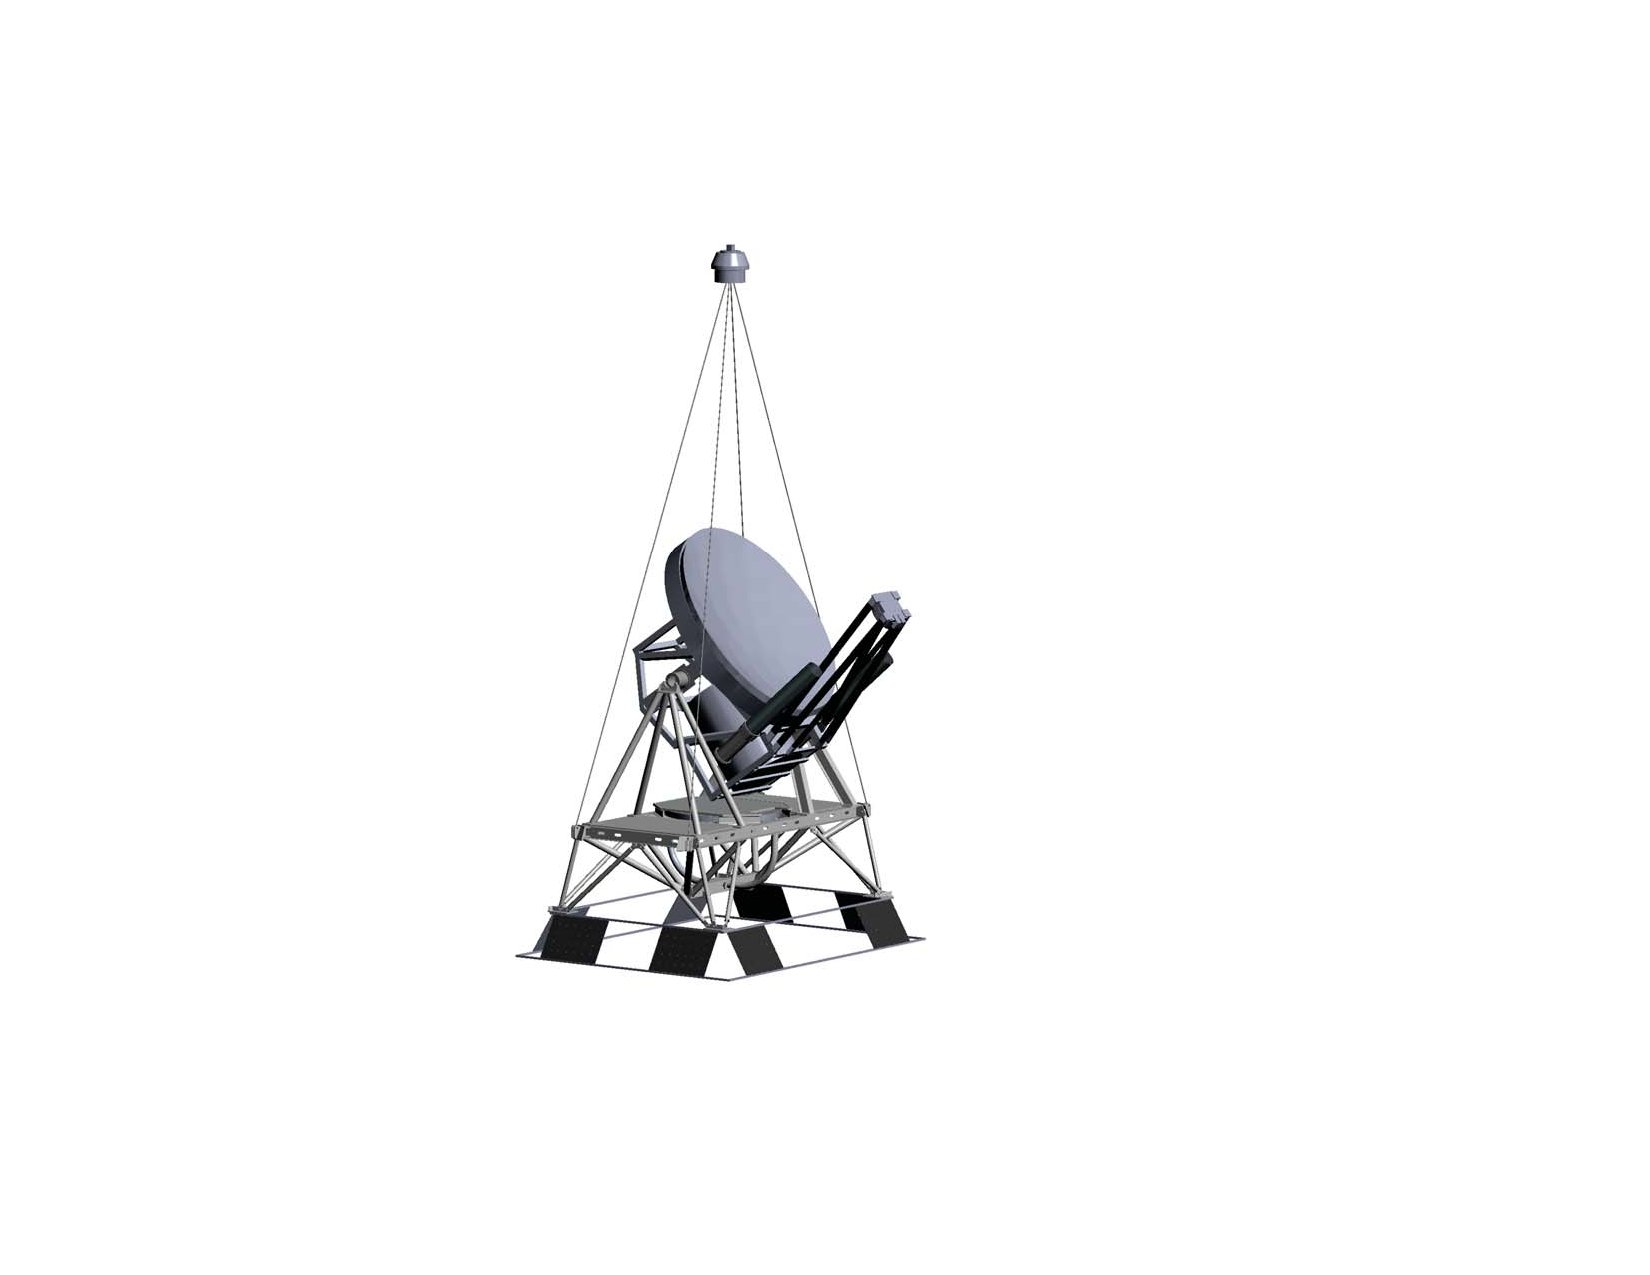
\includegraphics[height=4.5in]{ICarIS_gondola.pdf}
     \end{center}
   \end{minipage} &
   \begin{minipage}{3.5in} \vspace{-.2in}
     \begin{center} \hspace{+0.79in}
      \captionbaseline\caption{\small A Solidworks rendering of the \name\ telescope
showing the off-axis optical design and the approximate size and
location of the cryostat and star cameras.  The Sun shields are not
shown.  The structure is based on the proven \blast\ design.  The
frame will be made from carbon fiber and aluminum.  The upper part of
the gondola supporting the primary has been redesigned slightly from
the \blast\ architechture to support the larger off-axis \D\ mirror.}
       \label{fig:Gondola} 
       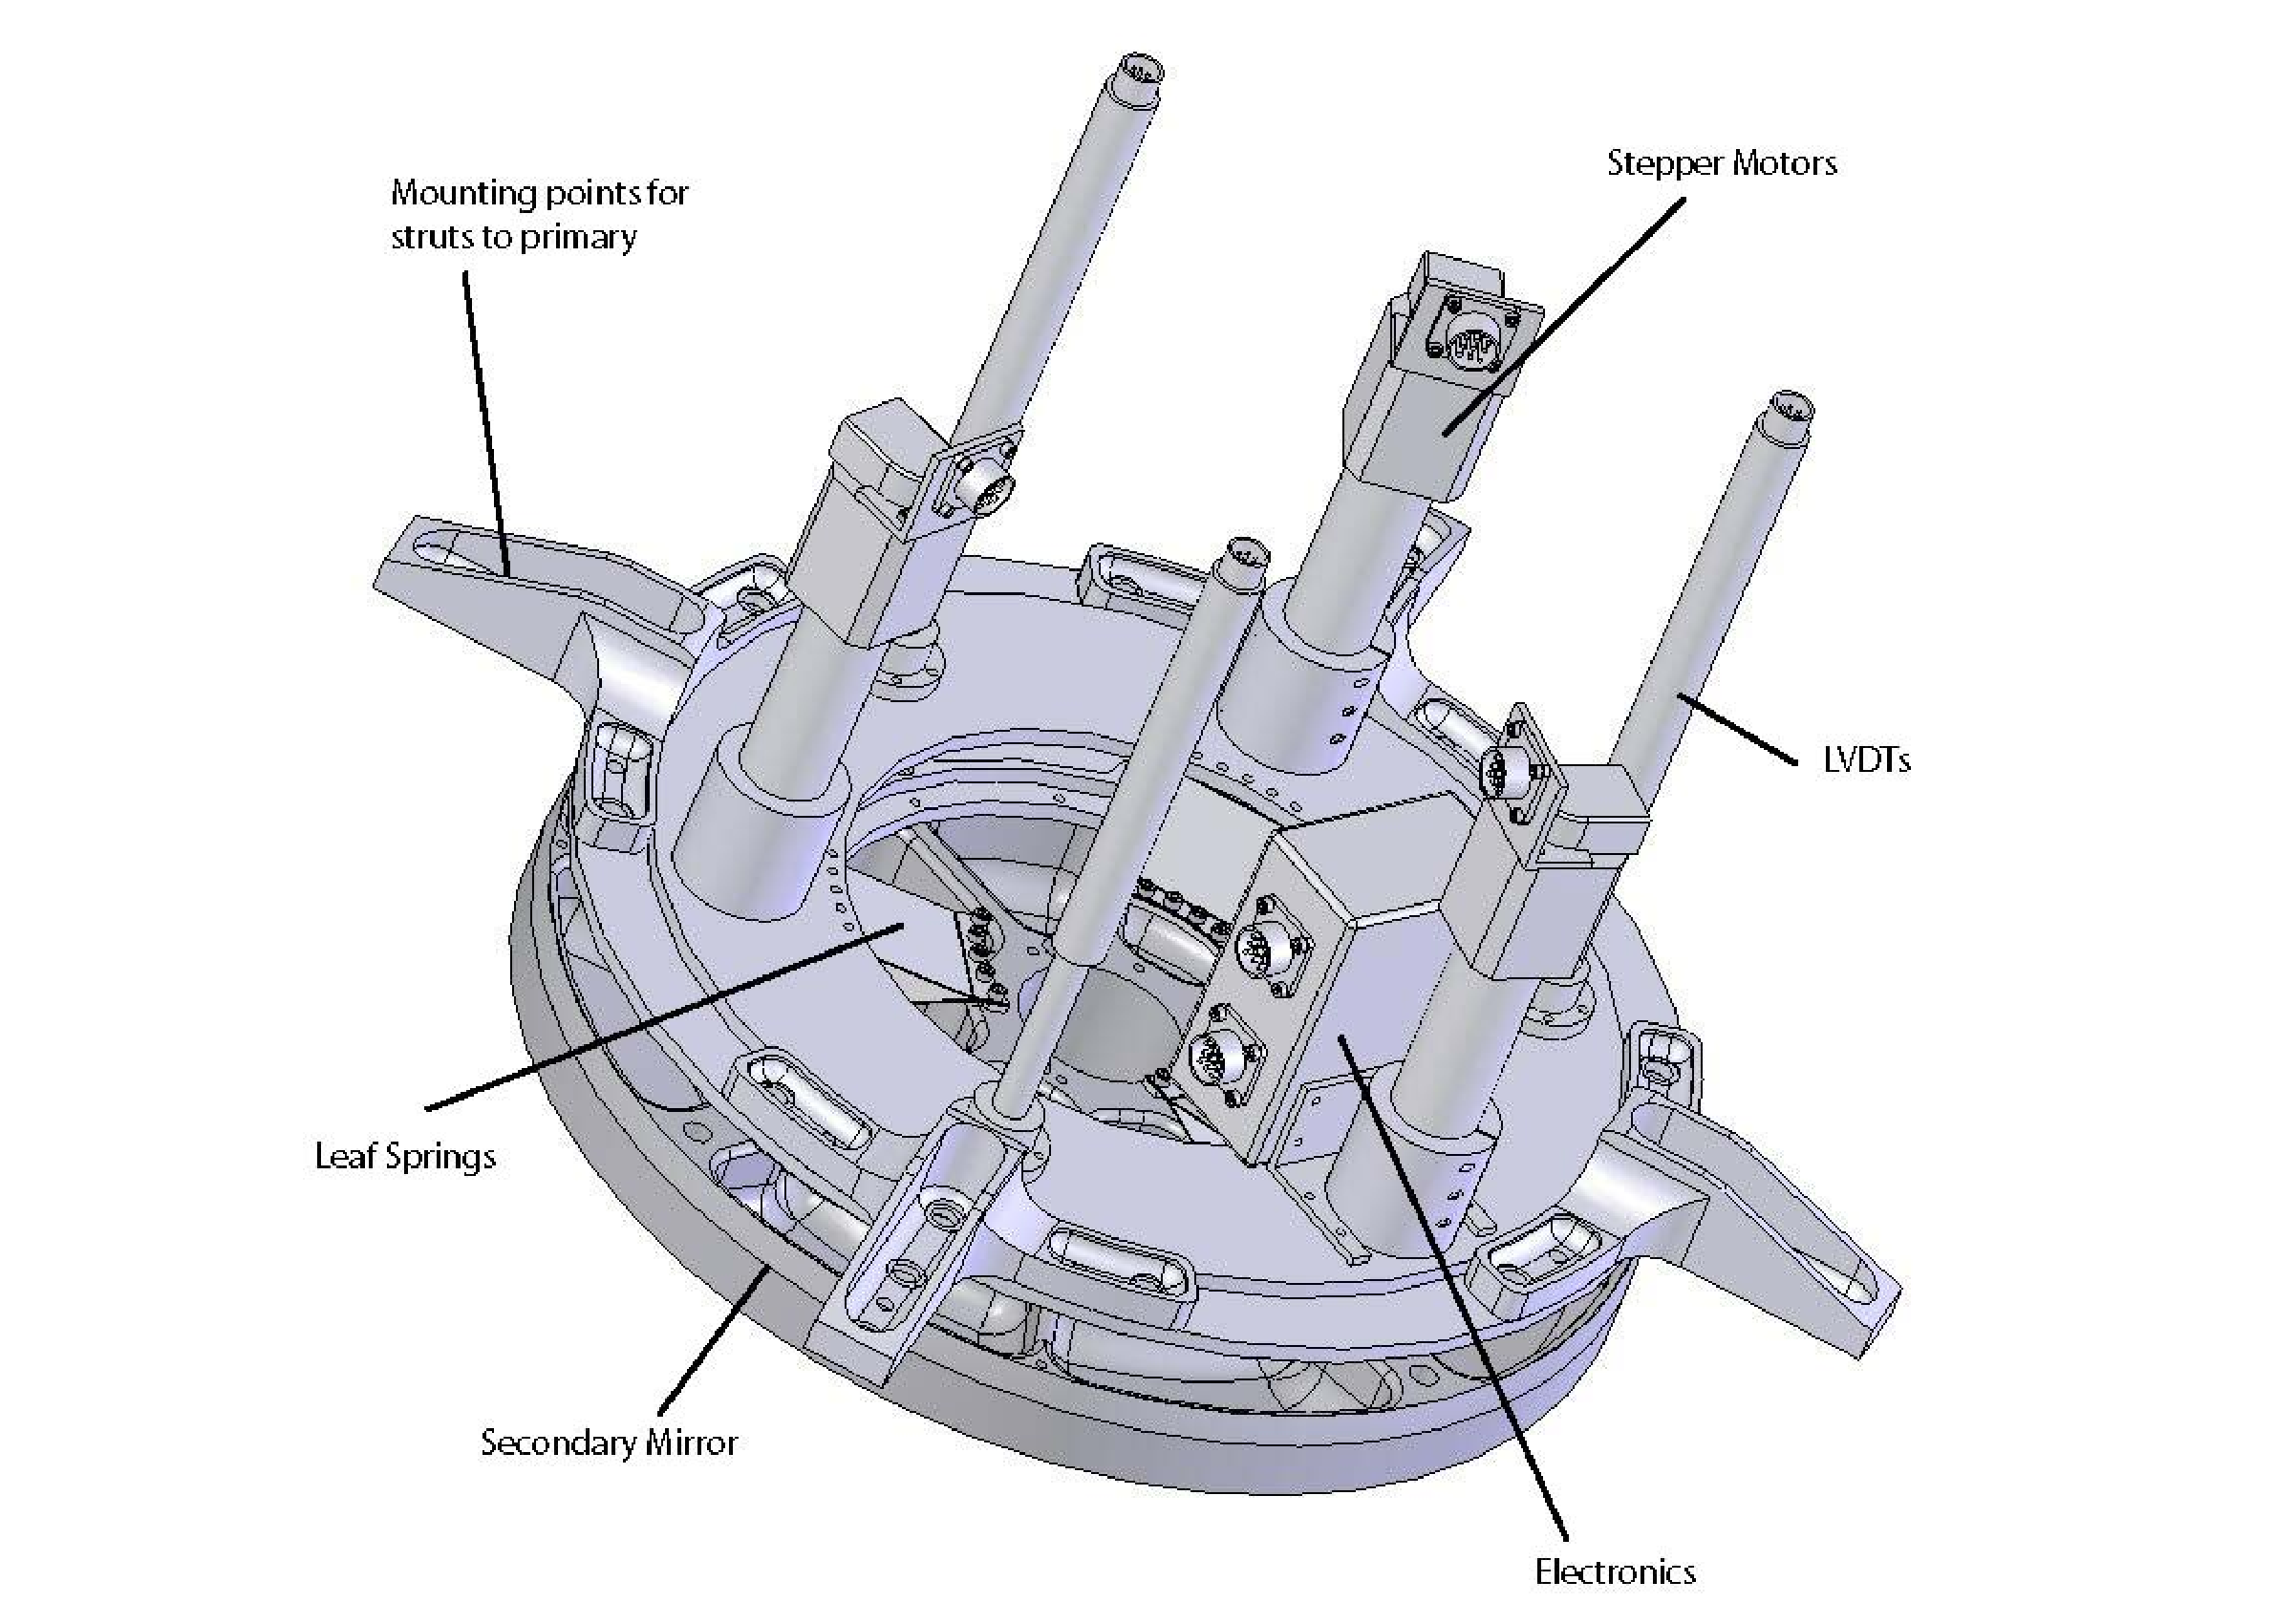
\psfig{file=secondary.pdf,angle=0, width=2.3in}
       \captionbaseline\caption {\small A rendering of the \blast\ secondary
	 positioning system.  \name\ will use the same system to
	 focus the off-axis secondary.  The system was successfully
	 tested during the \blast\ Antarctic flight in 2006.  It has
	 tip/tilt and positional accuracy (in one dimension) of
	 3~\mum.}
       \label{fig:SecondaryPositioning} 
     \end{center}
   \end{minipage}
 \end{tabular}
\end{figure}

\subsection{Cryogenics} 
 
The \name\ receiver consists of an optical cavity inside a long
hold-time liquid-nitrogen and liquid-helium cryostat.  Both the
nitrogen and helium are maintained at slightly more than 15~psi during
the flight to minimize loss due to pressure drop at altitude.  A pumped pot maintains a 1~K stage with 20~mW of cooling power, which contains the entire spectrometer.  The detectors are cooled with a series of pumped $^3$He/$^4$He sorption fridges, which back a commercially available adiabatic demagnetization refigerator (ADR) to achieve a final temperature of 150 mK.
A two-stage $^3$He refrigerator (designed and manufactured at Penn) provides a
300~mK sink during flight with $30\,\mu$W of cooling power for 3~days.  It is backed and cycled by a $^4$He stage.  It can be recycled within
2~hrs.  Our groups have built over ten
receivers operating at temperatures from 50 to 300~mK, including an ADR for Z-Spec.

\subsection{Pointing and System} 
\label{sec:Observing} 

The \name\ gondola and pointing system is designed around the
successful \blast\ heritage.  The gondola is shown in Figure
\ref{fig:Gondola}.  It consists of a precision-pointed inner frame
(composed of the primary, secondary, near-field baffle, and cryostat)
supported by an external gondola.  The outer frame is pointed in
azimuth by a flywheel and an active pivot. The inner frame has an
elevation mount with direct-drive servo motors driving it relative to
the outer frame.  Balance of the inner frame is maintained by pumping
liquid from the bottom of the frame to the top to compensate for
cryogen boil-off.

The pointing system design is driven by the requirement of high
in-flight accuracy, with an absolute accuracy of half a beam, and
reconstructed accuracy $<$3\arcsec.  The \blast\ Antarctic flight
obtained a pointing reconstruction of $\approx 3$\arcsec\ at $1\sigma$
for small (1 degree) scans \Citep{pascale08}.  The absolute in-flight
pointing error was about 1\arcmin.  By improving the rigidity of the
inner frame, and by not requiring large motions, we expect to be able
to obtain better absolute in-flight pointing accuracy for \name.

The attitude determination system uses an array of pointing sensors
including two sophisticated star cameras, two sets of fast, low-drift
gyroscopes, a quad-GPS system, a digital Sun sensor, encoders, tilt
sensors, and a magnetometer.  The software is written to take full
advantage of the abilities of each sensor in a hierarchical scheme
where the fast, high-drift sensors (gyros) are continuously updated by
the slower, absolute sensors (star cameras) and is robust against
sensor failure.
%The software is capable
%of determining the quality of the data from each sensor and
%automatically shifts to the next available sensor if there is a
%problem.  
Optical encoders report the relative position of the inner frame to
the outer frame.  Motion sensing for the inner frame is provided by
two sets of three orthogonally-mounted, high bandwidth gyroscopes.

The absolute pointing sensors are two integrating star cameras
\Citep{rex06} that are mounted above the receiver on the inner frame.
Each star camera has an internal computer that calculates a real-time
pointing solution at 1~Hz by comparing measured star separations with
an on-board catalog of stars.  The cameras are capable of dead
reckoning.  The two cameras run independently, providing failsafe
redundancy.
%This redundancy provides a
%failsafe backup and continuously measures the precision of the star
%camera pointing solution.  
The camera system has been tested extensively on the ground and has
flown four times on balloon payloads (three times on \blast\ and once
on the x-ray telescope InFOC$\mu$S).  
%The star cameras can identify
%magnitude 8 stars with an integration time of 300~ms in typical
%daytime float conditions.  
A comparison of simultaneous pointing solutions from both cameras
gives an rms uncertainty of $<$2\arcsec.  To meet the absolute
pointing requirements for \name, we will reduce the field of view of
the cameras by a factor of two and use new CCDs with enhanced quantum
efficiency that roughly doubles the sensitivity in the far red (where
\name\ uses them).  This will allow us to obtain high-accuracy,
continuously updated pointing solutions for our observations.


